\documentclass[11pt,a4paper,twoside]{article}

\usepackage[T1]{fontenc}
\usepackage{lmodern}
\usepackage[
  inner=2cm,
  outer=1.6cm,
  top=1.65cm,
  bottom=1.7cm,
  headheight=16pt,
  footskip=24pt
]{geometry}
\usepackage{microtype}
\usepackage{tabularx}
\usepackage{array}
\usepackage{enumitem}
\usepackage{titlesec}
\usepackage{fancyhdr}
\usepackage{hyperref}
\usepackage{amsmath}
\usepackage{tikz}
\usetikzlibrary{arrows.meta,positioning}

\hypersetup{
  hidelinks,
  pdftitle={Voice of the Customer Analytics},
  pdfsubject={Cognitive Computing Application Report},
  pdfkeywords={voice of the customer, natural language processing, sentiment analysis, cognitive computing}
}

\pagestyle{fancy}
\fancyhf{}
\fancyhead[LO,RE]{\footnotesize\scshape Cognitive Computing}
\fancyhead[RO,LE]{\footnotesize Voice of the Customer Analytics}
\fancyfoot[C]{\small\thepage\ of 10}
\renewcommand{\headrulewidth}{0pt}
\renewcommand{\footrulewidth}{0pt}

\fancypagestyle{plain}{
  \fancyhf{}
  \fancyfoot[C]{\small\thepage\ of 10}
  \renewcommand{\headrulewidth}{0pt}
  \renewcommand{\footrulewidth}{0pt}
}

\titleformat{\section}
  {\Large\bfseries}
  {\thesection.}{0.55em}{}
\titleformat{\subsection}
  {\normalsize\bfseries}
  {\thesubsection}{0.5em}{}
\titlespacing*{\section}{0pt}{0.5em}{0.42em}
\titlespacing*{\subsection}{0pt}{0.65em}{0.2em}

\setlength{\parindent}{0pt}
\setlength{\parskip}{0.42em}
\setlist[itemize]{leftmargin=1.35em,itemsep=0.18em,topsep=0.2em}
\setlist[enumerate]{leftmargin=1.45em,itemsep=0.18em,topsep=0.2em}
\renewcommand{\arraystretch}{1.22}
\setlength{\arrayrulewidth}{0.45pt}
\setlength{\tabcolsep}{5pt}
\newcolumntype{Y}{>{\raggedright\arraybackslash}X}
\newcolumntype{C}{>{\centering\arraybackslash}X}
\raggedbottom

\tikzset{
  flowbox/.style={
    draw=black,
    rounded corners=1.5pt,
    align=center,
    text width=3.15cm,
    minimum height=1.1cm,
    inner sep=4pt,
    font=\small
  },
  smallbox/.style={
    draw=black,
    rounded corners=1.2pt,
    align=center,
    text width=2.55cm,
    minimum height=0.82cm,
    inner sep=3pt,
    font=\footnotesize
  },
  widebox/.style={
    draw=black,
    rounded corners=1pt,
    align=center,
    text width=14.8cm,
    minimum height=0.58cm,
    inner xsep=4pt,
    inner ysep=2.5pt,
    font=\footnotesize
  },
  phasebox/.style={
    draw=black,
    rounded corners=1.2pt,
    align=center,
    text width=3.25cm,
    minimum height=1.05cm,
    inner sep=4pt,
    font=\footnotesize
  },
  flowarrow/.style={
    -{Stealth[length=2mm]},
    line width=0.5pt
  },
  returnarrow/.style={
    -{Stealth[length=1.7mm]},
    line width=0.45pt
  }
}

\begin{document}
\thispagestyle{plain}

\begin{center}
\vspace*{0.2em}
{\small\scshape Cognitive Computing Application Report\par}
\vspace{0.65em}
{\fontsize{25}{30}\selectfont\bfseries Voice of the Customer Analytics\par}
\vspace{0.3em}
{\large\itshape An NLP system for converting customer language into accountable business decisions\par}
\vspace{0.6em}
{\small
\textbf{Selected application:} Voice of the Customer Analytics\par
\textbf{Domain:} Retail, e-commerce, banking, telecom, travel, and digital services\par
\textbf{Document format:} Ten-page duplex-ready report\par}
\end{center}

\section{Business Problem}

\subsection{Executive Context}

Customers describe defects, service failures, unmet needs, and purchase motives through reviews, surveys, support chats, call transcripts, email, and public posts. A large organization may collect thousands of comments each day, yet managers often depend on star ratings, manually prepared summaries, or a small sample of memorable complaints. Those methods hide the target of an opinion. A low rating can refer to delivery, price, usability, staff conduct, or the product itself.

Voice of the Customer (VoC) analytics applies natural language processing (NLP) to organize this language around business questions. The system identifies what customers discuss, measures how they feel about each aspect, detects changes over time, and links every summary to supporting records. Product, operations, and customer-experience teams gain a common evidence base instead of maintaining separate spreadsheets and channel-specific dashboards.

\subsection{Problem Definition}

The proposed application addresses four connected problems:

\begin{itemize}
  \item \textbf{Scale:} feedback arrives faster than analysts can read, label, and route it.
  \item \textbf{Fragmentation:} channels use different identifiers, formats, rating scales, and retention rules.
  \item \textbf{Context:} one comment can praise a feature, criticize delivery, and request a refund.
  \item \textbf{Actionability:} a sentiment score does not identify the cause, owner, urgency, or affected customer group.
\end{itemize}

The first release should support a limited product line and answer three questions: Which themes are rising? Which customer or product segments experience them? Which team should investigate first? The organization should judge success through model quality, analyst adoption, detection lead time, and the share of verified issues that receive an owner.

\subsection{System Overview}

\begin{center}
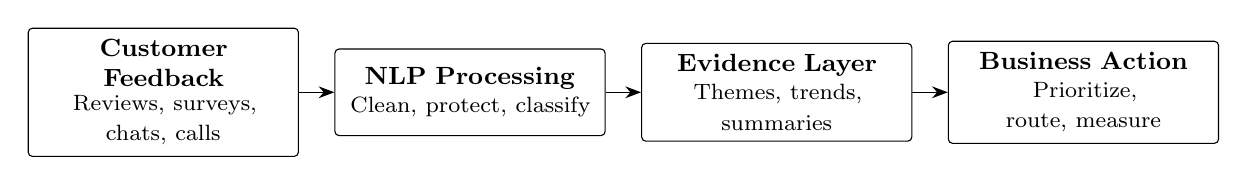
\begin{tikzpicture}[node distance=0.45cm]
  \node[flowbox] (sources) {\textbf{Customer Feedback}\\[-0.1em]\footnotesize Reviews, surveys,\\chats, calls};
  \node[flowbox, right=of sources] (process) {\textbf{NLP Processing}\\[-0.1em]\footnotesize Clean, protect, classify};
  \node[flowbox, right=of process] (insights) {\textbf{Evidence Layer}\\[-0.1em]\footnotesize Themes, trends, summaries};
  \node[flowbox, right=of insights] (action) {\textbf{Business Action}\\[-0.1em]\footnotesize Prioritize, route, measure};
  \draw[flowarrow] (sources) -- (process);
  \draw[flowarrow] (process) -- (insights);
  \draw[flowarrow] (insights) -- (action);
\end{tikzpicture}

\vspace{0.1em}
{\small\textbf{Figure 1.} High-level Voice of the Customer workflow.}
\end{center}

\newpage

\section{Business Decisions and Use Cases}

\subsection{Stakeholders and Decisions}

A VoC platform creates value only when teams connect its outputs to named decisions. Product managers need feature evidence, service leaders need failure patterns, and compliance teams need controlled access to sensitive records. The following table defines the primary users and the questions each group should answer.

\begin{tabularx}{\textwidth}{|>{\raggedright\arraybackslash}p{3.05cm}|Y|Y|}
\hline
\textbf{Stakeholder} & \textbf{Decision supported} & \textbf{Required evidence} \\ \hline
Product management & Select defects, usability issues, and feature requests for the roadmap & Aspect volume, sentiment, affected versions, representative comments \\ \hline
Customer support & Route urgent cases and improve scripts or self-service content & Intent, emotion, severity, repeat contacts, resolution outcome \\ \hline
Operations & Investigate delivery, outage, refund, and process failures & Theme growth, region, partner, timestamp, linked operational event \\ \hline
Marketing and research & Compare customer language across segments and campaigns & Segment distribution, purchase motive, topic mix, verbatim evidence \\ \hline
Risk and compliance & Review sensitive complaints and confirm lawful data use & PII status, consent basis, access log, retention and deletion record \\ \hline
\end{tabularx}

\subsection{Priority Use Cases}

\textbf{Emerging-issue detection.} The system compares current theme volume with a rolling baseline. An alert should include the growth rate, sample size, affected products, and a small set of source comments. An analyst confirms whether the increase reflects a real issue, a campaign, duplicate records, or a channel outage.

\textbf{Release comparison.} Product teams compare aspect-level sentiment before and after a software, packaging, policy, or pricing change. The analysis should control for channel and customer mix so a new survey campaign does not look like a product failure.

\textbf{Complaint routing.} The platform assigns a proposed owner from aspect, intent, severity, product, and location. Human reviewers approve safety, legal, account-closure, and high-value customer cases before the platform creates a ticket.

\textbf{Customer journey analysis.} When policy permits record linkage, teams can connect feedback to order, delivery, return, support, and renewal events. This view distinguishes a product defect from a poor recovery experience.

\subsection{Success Measures}

The pilot should establish baseline values before deployment. Operational measures include median review hours per reporting cycle, time from first complaint to verified alert, time from alert to owner, and closure rate. Model measures include macro F1, calibration error, summary faithfulness, and subgroup performance. Adoption measures include analyst override rate, evidence-link usage, and the number of decisions recorded against an insight.

The organization should avoid using overall sentiment as the main success measure. Sentiment can fall after the team expands feedback collection to dissatisfied customers even when the service improves. A credible evaluation connects each insight to an action and then measures the operational or customer result.

\newpage

\section{NLP Techniques Used}

A production VoC system combines several NLP tasks because no single classifier captures topic, target, intensity, intent, and cause.

\begin{tabularx}{\textwidth}{|>{\raggedright\arraybackslash}p{3.15cm}|Y|Y|}
\hline
\textbf{Technique} & \textbf{Role in the system} & \textbf{Typical output} \\ \hline
Normalization and language detection & Repair encoding, separate sentences, preserve negation, identify language, and standardize channel-specific abbreviations & Clean text, language code, quality flags \\ \hline
PII and entity extraction & Mask personal data and identify products, versions, locations, partners, and service stages & Protected text and typed entities \\ \hline
Aspect-based sentiment analysis & Link positive, neutral, or negative opinion to a specific target instead of the whole document \cite{hu2004,pontiki2014} & Aspect, polarity, intensity, confidence \\ \hline
Emotion and intent classification & Detect frustration, delight, urgency, complaint, cancellation, request, compliment, or question & Multi-label emotion and intent scores \\ \hline
Embedding and topic discovery & Group semantically related comments and surface themes that the fixed taxonomy does not cover & Cluster identifier, theme label, novelty score \\ \hline
Evidence-grounded summarization & Produce a short theme account and retrieve comments that support each statement & Summary, citations, sample size, exceptions \\ \hline
\end{tabularx}

\subsection{Aspect and Sentiment Modeling}

Aspect extraction identifies the entity or service element that a customer evaluates. In ``the camera is sharp but the battery drains overnight,'' the model should assign positive sentiment to camera quality and negative sentiment to battery life. Sequence labeling can mark explicit spans, while a domain taxonomy maps phrases such as ``dies by dinner'' to a battery-performance concept. Transformer encoders such as BERT provide a strong supervised foundation when the team fine-tunes them on domain labels \cite{devlin2019}.

The classifier should return calibrated probabilities rather than only a label. The application can auto-accept high-confidence routine records, send uncertain records to analysts, and force human review for high-severity intents. This design gives the business a controllable operating threshold.

\subsection{Theme Discovery and Summarization}

Embedding-based clustering groups paraphrases that keyword rules miss. Topic models such as latent Dirichlet allocation provide an interpretable baseline for broad themes \cite{blei2003}, while sentence embeddings support finer semantic clusters. Analysts should name, merge, and retire clusters; otherwise the theme inventory becomes inconsistent across reporting periods.

Summarization should start with retrieval. The system selects representative and contradictory comments, then creates a constrained summary from that evidence. Each sentence should link to source records, sample size, time window, and segment filters. A summary that lacks evidence should not appear in an executive dashboard.

\subsection{Multilingual and Noisy Text}

Customer language contains spelling variants, emojis, code-switching, sarcasm, and speech-recognition errors. The pipeline should preserve the original record, store normalized text separately, and route low-quality transcripts for review. Evaluation must report each supported language independently; a high English score cannot justify deployment for another language.

\newpage

\section{Reference Architecture}

The architecture separates collection, governance, model services, insight delivery, and business action. This separation lets the organization update a classifier without changing channel connectors or ticketing integrations.

\begin{center}
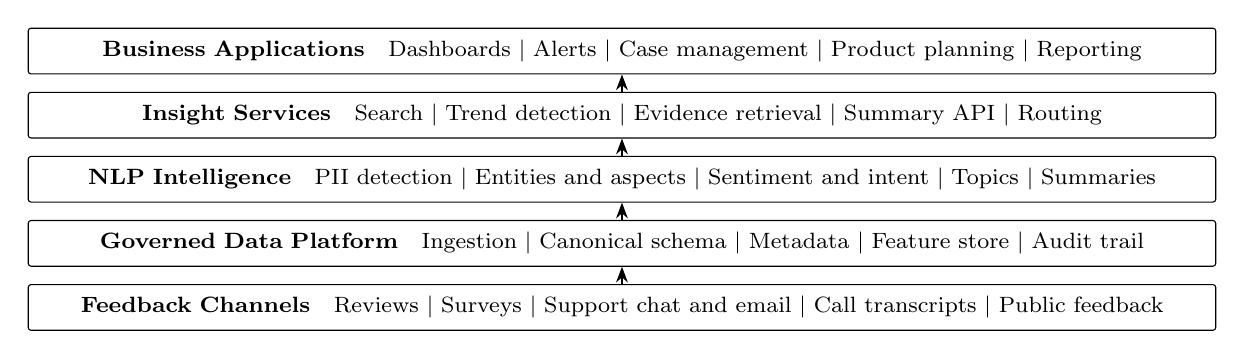
\begin{tikzpicture}[node distance=0.22cm]
  \node[widebox] (apps) {\textbf{Business Applications}\quad Dashboards \textbar\ Alerts \textbar\ Case management \textbar\ Product planning \textbar\ Reporting};
  \node[widebox, below=of apps] (delivery) {\textbf{Insight Services}\quad Search \textbar\ Trend detection \textbar\ Evidence retrieval \textbar\ Summary API \textbar\ Routing};
  \node[widebox, below=of delivery] (nlp) {\textbf{NLP Intelligence}\quad PII detection \textbar\ Entities and aspects \textbar\ Sentiment and intent \textbar\ Topics \textbar\ Summaries};
  \node[widebox, below=of nlp] (data) {\textbf{Governed Data Platform}\quad Ingestion \textbar\ Canonical schema \textbar\ Metadata \textbar\ Feature store \textbar\ Audit trail};
  \node[widebox, below=of data] (channels) {\textbf{Feedback Channels}\quad Reviews \textbar\ Surveys \textbar\ Support chat and email \textbar\ Call transcripts \textbar\ Public feedback};

  \draw[flowarrow] (channels.north) -- (data.south);
  \draw[flowarrow] (data.north) -- (nlp.south);
  \draw[flowarrow] (nlp.north) -- (delivery.south);
  \draw[flowarrow] (delivery.north) -- (apps.south);
\end{tikzpicture}

\vspace{0.1em}
{\small\textbf{Figure 2.} Layered reference architecture for the VoC platform.}
\end{center}

\subsection{Component Responsibilities}

\textbf{Channel connectors} collect approved fields from review platforms, survey tools, customer-support systems, speech transcription services, and operational databases. Each connector records source, ingestion time, consent basis, and a stable source identifier. Deduplication occurs before model inference.

\textbf{The governed data platform} stores raw records under restricted access and publishes protected records through a canonical schema. It manages retention, deletion, data quality, annotation versions, and links to product or operational metadata. Analysts work with masked text unless a controlled investigation requires the source.

\textbf{NLP intelligence services} expose versioned interfaces for language detection, PII masking, entity extraction, aspect sentiment, intent, embeddings, clustering, and summarization. A model registry links each prediction to model, taxonomy, prompt, and dataset versions.

\textbf{Insight services} aggregate record-level predictions into trends. They enforce minimum sample sizes, retrieve evidence, detect unusual volume, and calculate priority scores. These services should return structured results rather than formatted dashboard text so multiple applications can reuse them.

\textbf{Business applications} present dashboards, alerts, search, tickets, and planning views. Each application records analyst confirmation, correction, owner, and outcome. Those decisions return to the training and governance workflow.

\subsection{Data and Control Flow}

The data path moves upward from channels to action, while control signals move downward. Governance rules determine permitted fields, model thresholds determine review queues, and analyst corrections update labels. Authentication should use service identities with least privilege. Audit records should capture who viewed raw text, who changed a label, which evidence supported a summary, and which action followed an alert.

The design should process routine feedback in batches and urgent channels through near-real-time queues. Batch processing controls cost for historical analysis; event processing supports safety, fraud, outage, and account-access complaints that require faster routing.

\newpage

\section{Dataset Required}

\subsection{Data Sources and Schema}

The strongest dataset combines first-party feedback with product, channel, customer-segment, and operational context. Public corpora help test code, but internal data defines the taxonomy and operating conditions.

\begin{tabularx}{\textwidth}{|>{\raggedright\arraybackslash}p{2.75cm}|Y|Y|}
\hline
\textbf{Source} & \textbf{Text and labels} & \textbf{Required metadata} \\ \hline
Reviews and surveys & Free-text feedback, rating, satisfaction score, optional reason code & Product, version, date, channel, language, locale \\ \hline
Support interactions & Chat, email, ticket notes, call transcript, disposition & Queue, contact reason, resolution, handling time, repeat contact \\ \hline
Public feedback & Approved app-store, forum, and social posts & Source, post date, engagement, collection and consent basis \\ \hline
Operational records & Delivery, outage, return, refund, defect, or policy event & Event type, timestamp, product, partner, region \\ \hline
Annotation records & Aspect, target span, sentiment, emotion, intent, severity, uncertainty & Annotator, guideline version, adjudication, quality status \\ \hline
\end{tabularx}

\subsection{Sampling and Annotation}

A practical pilot can use 40,000--60,000 recent comments sampled across products, channels, rating levels, languages, regions, and customer segments. The team should double-label a balanced subset of about 10,000 records. An adjudicator resolves disagreements and updates the guideline when annotators interpret a category differently.

The schema should permit multiple aspects and sentiments in one comment. Annotators need explicit values for sarcasm, mixed sentiment, missing context, and unusable transcript quality. Cohen's kappa or Krippendorff's alpha measures agreement, but the team should also inspect disagreement by category. Low agreement often signals an unclear taxonomy rather than careless annotators.

The split must follow customer and time boundaries. All records from one case or customer belong in one split, and the test period should occur after the training period. This method limits leakage and measures drift. Rare, costly issues need deliberate sampling for training and separate prevalence-aware reporting during evaluation.

\subsection{Dataset Lifecycle}

\begin{center}
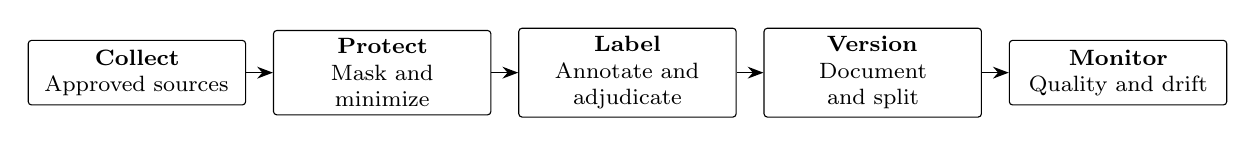
\begin{tikzpicture}[node distance=0.34cm]
  \node[smallbox] (collect) {\textbf{Collect}\\Approved sources};
  \node[smallbox, right=of collect] (protect) {\textbf{Protect}\\Mask and minimize};
  \node[smallbox, right=of protect] (label) {\textbf{Label}\\Annotate and adjudicate};
  \node[smallbox, right=of label] (version) {\textbf{Version}\\Document and split};
  \node[smallbox, right=of version] (monitor) {\textbf{Monitor}\\Quality and drift};
  \draw[flowarrow] (collect) -- (protect);
  \draw[flowarrow] (protect) -- (label);
  \draw[flowarrow] (label) -- (version);
  \draw[flowarrow] (version) -- (monitor);
\end{tikzpicture}

\vspace{0.1em}
{\small\textbf{Figure 3.} Governed dataset lifecycle.}
\end{center}

\subsection{Governance Requirements}

The data owner should publish a dataset card that records provenance, sampling, label definitions, agreement, exclusions, retention, known gaps, and permitted uses \cite{gebru2021}. The platform must support deletion requests and prevent removed records from returning through cached training files. Public feedback requires the same legal and ethical review as first-party data; public visibility does not remove purpose and retention obligations.

Public datasets such as the Amazon review corpus can support prototyping because they contain product text, ratings, and categories at scale \cite{ni2019}. They cannot validate the company's service taxonomy, language mix, policy constraints, or customer journey. Final acceptance testing should use protected internal records drawn from the intended deployment period.

\newpage

\section{Model Development and Evaluation}

\subsection{Development Workflow}

\begin{center}
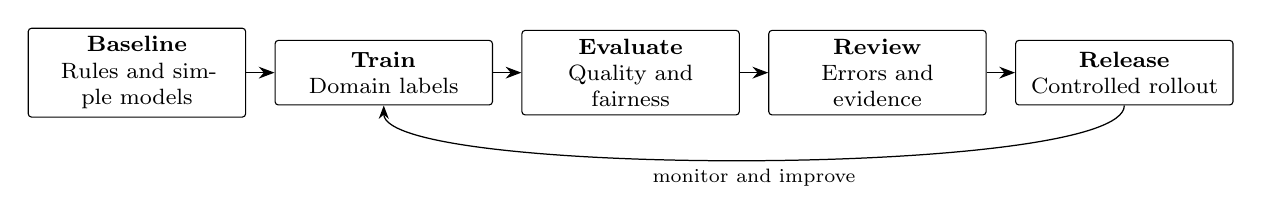
\begin{tikzpicture}[node distance=0.36cm]
  \node[smallbox] (baseline) {\textbf{Baseline}\\Rules and simple models};
  \node[smallbox, right=of baseline] (train) {\textbf{Train}\\Domain labels};
  \node[smallbox, right=of train] (evaluate) {\textbf{Evaluate}\\Quality and fairness};
  \node[smallbox, right=of evaluate] (review) {\textbf{Review}\\Errors and evidence};
  \node[smallbox, right=of review] (release) {\textbf{Release}\\Controlled rollout};
  \draw[flowarrow] (baseline) -- (train);
  \draw[flowarrow] (train) -- (evaluate);
  \draw[flowarrow] (evaluate) -- (review);
  \draw[flowarrow] (review) -- (release);
  \draw[returnarrow] (release.south) to[out=-90,in=-90,looseness=0.25]
    node[below, font=\scriptsize]{monitor and improve} (train.south);
\end{tikzpicture}

\vspace{0.05em}
{\small\textbf{Figure 4.} Model development, review, and release workflow.}
\end{center}

The first benchmark should include transparent baselines: keyword rules, logistic regression with n-grams, and a simple topic model. These baselines expose data problems and set a minimum standard. The team can then compare transformer classifiers, embedding models, and constrained summarization methods against the same fixed test set.

\subsection{Evaluation Measures}

\begin{tabularx}{\textwidth}{|>{\raggedright\arraybackslash}p{3.05cm}|Y|Y|}
\hline
\textbf{Measure} & \textbf{Question answered} & \textbf{Reporting requirement} \\ \hline
Macro precision, recall, and F1 & Does the model perform across common and rare labels? & Report by aspect, intent, language, channel, and segment \\ \hline
Calibration error & Does stated confidence match observed correctness? & Reliability plot and threshold analysis \\ \hline
Cluster coherence and stability & Do discovered themes represent consistent language over time? & Analyst rating, overlap, and period-to-period matching \\ \hline
Summary faithfulness & Does each claim follow from retrieved evidence? & Sentence-level evidence check and unsupported-claim rate \\ \hline
Routing precision & Does the proposed owner match the approved owner? & Precision by team, severity, and escalation type \\ \hline
Operational lift & Does the system improve the workflow? & Review time, detection lead time, ownership time, closure rate \\ \hline
\end{tabularx}

\subsection{Error Analysis and Release Gates}

Reviewers should examine false positives, false negatives, low-confidence cases, subgroup gaps, and disagreements between the model and analysts. A confusion matrix can reveal overlapping categories such as ``delivery delay'' and ``order status.'' Evidence review can expose summaries that overstate a minority view. Local explanation methods can help analysts inspect influential words, but they do not replace counterfactual tests or source evidence \cite{ribeiro2016}.

The release process should define gates. A model must meet minimum class-level recall for safety or account-access issues, stay within approved subgroup gaps, produce calibrated confidence, and pass privacy tests. The team should create a model card with training scope, evaluation results, limitations, thresholds, and excluded uses \cite{mitchell2019}. A failed gate returns the model to data review rather than to production.

\newpage

\section{Expected Outcomes}

\subsection{System Outputs}

The platform should produce five traceable outputs: an aspect-sentiment dashboard, emerging-theme alerts, segment comparisons, evidence-grounded summaries, and routed cases. Each output must display the time window, filters, sample size, model version, confidence, and source comments. Analysts should be able to correct labels and mark an insight as confirmed, dismissed, merged, or assigned.

\begin{tabularx}{\textwidth}{|>{\raggedright\arraybackslash}p{3.05cm}|Y|Y|}
\hline
\textbf{Outcome} & \textbf{Operational use} & \textbf{Measure} \\ \hline
Faster issue discovery & Alert owners when a theme rises above its expected baseline & Detection lead time and valid-alert rate \\ \hline
Better prioritization & Rank issues by volume, severity, growth, reach, and customer value & Time to owner and accepted-priority rate \\ \hline
Product learning & Compare aspect sentiment and language before and after a release & Change by aspect, product version, and segment \\ \hline
Analyst efficiency & Replace repetitive reading with review of evidence clusters & Review hours per reporting cycle \\ \hline
Closed-loop service & Route urgent records and track the action taken & Escalation precision, closure rate, repeat contact \\ \hline
\end{tabularx}

\subsection{Priority Model}

The platform can combine normalized business signals into a transparent priority score:

\[
P = w_v V + w_s S + w_g G + w_r R + w_c C,
\]

where \(V\) is volume, \(S\) is severity, \(G\) is growth above baseline, \(R\) is customer or operational reach, and \(C\) is expected cost or customer value. Business owners should approve the weights and view the component values. The score should rank investigation candidates; it should not make refunds, account actions, or safety decisions.

\subsection{Measurement Design}

The pilot should compare the assisted workflow with the previous manual process. During an initial shadow period, analysts receive system insights but follow the existing process. The team records whether the system found a verified issue earlier and whether evidence supported the proposed owner. During the controlled-use period, selected teams act on insights and record disposition, resolution, and outcome.

Customer metrics need careful interpretation. An increase in complaint volume may reflect broader collection, a successful request for feedback, or a genuine failure. The evaluation should use comparable segments and time windows. Product changes can use pre/post analysis with a control product or region when available.

\subsection{Example Insight Record}

An actionable record might state: ``Battery-drain complaints for mobile app version 8.4 increased from a weekly baseline of 1.8\% to 5.6\% across 642 English-language reviews. Most comments mention background location use. The model retrieved 25 representative comments and 6 contradictory comments. Product Mobile owns the investigation.'' This record gives the owner enough evidence to reproduce the finding. A label such as ``negative sentiment: 0.91'' does not.

Expected benefits include earlier fault detection, clearer ownership, faster reporting, and a searchable history of customer evidence. The organization should claim these benefits only after the pilot measures them.

\newpage

\section{Challenges}

VoC analytics combines difficult language problems with privacy, security, and organizational risks. The project plan should treat these risks as design requirements.

\begin{tabularx}{\textwidth}{|>{\raggedright\arraybackslash}p{3.05cm}|Y|Y|}
\hline
\textbf{Challenge} & \textbf{Failure mode} & \textbf{Control} \\ \hline
Ambiguous language & Sarcasm, comparison, implied targets, and mixed sentiment produce wrong labels & Uncertainty class, domain examples, human review \\ \hline
Uneven representation & Review writers and support users do not represent all customers & Coverage reporting, segment analysis, weighted sampling \\ \hline
Taxonomy drift & New products, policies, and slang make labels incomplete & Novelty detection, monthly taxonomy review, versioning \\ \hline
Manipulation and spam & Duplicate or coordinated posts create false trends & Deduplication, source reputation, anomaly checks \\ \hline
Privacy and security & Text exposes personal data or malicious instructions & Data minimization, PII masking, access control, input isolation \\ \hline
Unfaithful summaries & Generated text adds a claim that evidence does not support & Retrieval first, sentence citations, contradiction sampling, review \\ \hline
Organizational adoption & Teams receive insights without ownership or workflow integration & Named owners, ticket integration, decision and closure logs \\ \hline
\end{tabularx}

\subsection{Bias and Coverage}

Online reviews overrepresent customers motivated to post, and support channels overrepresent problems. Survey incentives, language availability, accessibility, and regional channel preferences also affect coverage. The dashboard should show who and what the dataset represents rather than presenting feedback as a census. Analysts should compare conclusions across channels and segments before escalating them.

Model evaluation must report errors for supported languages, regions, product groups, and high-impact intents. A single aggregate score can hide poor rare-class performance. Sentiment also varies by domain; words that signal approval in one context may indicate a defect in another \cite{liu2012}.

\subsection{Privacy, Security, and Governance}

Customer text can contain names, phone numbers, addresses, health information, financial data, credentials, or authentication details. The system should minimize collection, mask PII before annotation, encrypt stored records, restrict raw-text access, and log every privileged view. Retention and deletion rules must cover raw records, protected copies, embeddings, annotation exports, model prompts, and cached evidence.

Generative components should treat customer text as untrusted input. The application must separate instructions from retrieved content, restrict tools, validate outputs, and prevent summaries from exposing sensitive source text. The governance program can use the NIST AI Risk Management Framework as a structure for mapping, measuring, managing, and governing risk \cite{nist2023}.

\subsection{Trust and Human Oversight}

Analysts need source links, confidence, sample size, filters, model version, and counterexamples. They should be able to override labels without hiding disagreement. High-impact alerts require human approval, and the platform should record the reviewer, decision, reason, owner, and outcome. These records support audits and create training examples for later releases.

\newpage

\section{Future Improvements}

\subsection{Capability Roadmap}

\begin{enumerate}
  \item \textbf{Active learning:} select uncertain, novel, and high-impact records for labeling so analysts spend time on examples that improve coverage.
  \item \textbf{Multilingual analysis:} add language-specific evaluation, translation quality controls, and native-language review for high-impact themes.
  \item \textbf{Multimodal evidence:} analyze screenshots, product images, and audio quality when customers attach them to complaints.
  \item \textbf{Knowledge-grounded summaries:} retrieve product catalogs, policy versions, incident records, and resolved tickets before generating a summary.
  \item \textbf{Causal evaluation:} connect themes to controlled releases and operational events to distinguish correlation from a verified cause.
  \item \textbf{Personalized routing:} recommend an owner and next action from product responsibility, severity, service-level targets, and customer history while retaining human approval.
\end{enumerate}

\begin{center}
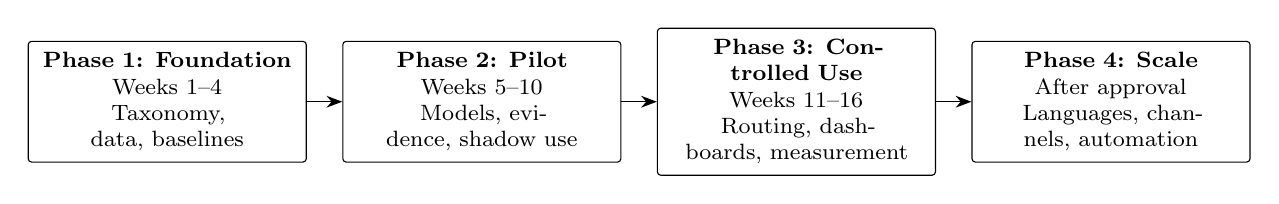
\begin{tikzpicture}[node distance=0.45cm]
  \node[phasebox] (p1) {\textbf{Phase 1: Foundation}\\Weeks 1--4\\Taxonomy, data, baselines};
  \node[phasebox, right=of p1] (p2) {\textbf{Phase 2: Pilot}\\Weeks 5--10\\Models, evidence, shadow use};
  \node[phasebox, right=of p2] (p3) {\textbf{Phase 3: Controlled Use}\\Weeks 11--16\\Routing, dashboards, measurement};
  \node[phasebox, right=of p3] (p4) {\textbf{Phase 4: Scale}\\After approval\\Languages, channels, automation};
  \draw[flowarrow] (p1) -- (p2);
  \draw[flowarrow] (p2) -- (p3);
  \draw[flowarrow] (p3) -- (p4);
\end{tikzpicture}

\vspace{0.1em}
{\small\textbf{Figure 5.} Recommended implementation roadmap.}
\end{center}

\subsection{Implementation Priorities}

\textbf{Phase 1} establishes data ownership, access controls, annotation guidelines, a limited aspect taxonomy, and baseline models. The team should select one product line with enough feedback and engaged business owners. This phase ends when the dataset passes quality review and the baselines produce reproducible results.

\textbf{Phase 2} trains domain models, adds evidence retrieval, and runs the system in shadow mode. Analysts compare its themes and alerts with their existing reports. The team studies errors, calibrates thresholds, and records which insights would have changed a decision.

\textbf{Phase 3} integrates approved alerts with case management and product planning. Selected teams act on insights, record disposition, and measure detection and ownership time. Governance reviewers approve any expansion in data, automation, or retention.

\textbf{Phase 4} adds languages, channels, multimodal evidence, and more automated routing only after the controlled pilot meets quality and risk gates. The program should prefer one reliable workflow over many dashboards that teams do not use.

\subsection{Continuous Improvement}

\begin{center}
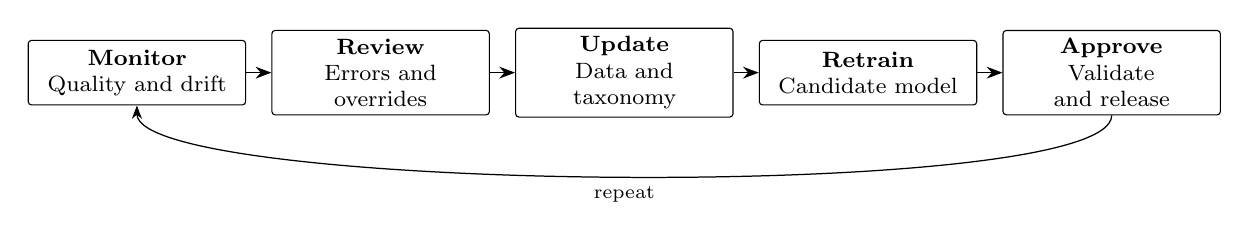
\begin{tikzpicture}[node distance=0.32cm]
  \node[smallbox] (monitor) {\textbf{Monitor}\\Quality and drift};
  \node[smallbox, right=of monitor] (review) {\textbf{Review}\\Errors and overrides};
  \node[smallbox, right=of review] (update) {\textbf{Update}\\Data and taxonomy};
  \node[smallbox, right=of update] (retrain) {\textbf{Retrain}\\Candidate model};
  \node[smallbox, right=of retrain] (approve) {\textbf{Approve}\\Validate and release};
  \draw[flowarrow] (monitor) -- (review);
  \draw[flowarrow] (review) -- (update);
  \draw[flowarrow] (update) -- (retrain);
  \draw[flowarrow] (retrain) -- (approve);
  \draw[returnarrow] (approve.south) to[out=-90,in=-90,looseness=0.23]
    node[below, font=\scriptsize]{repeat} (monitor.south);
\end{tikzpicture}

\vspace{0.05em}
{\small\textbf{Figure 6.} Human-supervised improvement cycle.}
\end{center}

A monthly operating review should examine drift, subgroup errors, alert precision, analyst overrides, summary faithfulness, and unresolved high-severity records. Quarterly governance review should approve taxonomy, retention, and automation changes. Each model release needs a rollback plan and a reproducible link to data, code, configuration, and evaluation results.

\newpage

\section{Conclusion and Recommendations}

Voice of the Customer analytics fits cognitive computing because it combines language understanding, learning, context, evidence, and human judgment. A useful system goes beyond positive and negative counts. It identifies the target of an opinion, discovers new themes, retrieves supporting records, and connects an insight to a responsible team.

The organization should begin with a governed pilot rather than an enterprise-wide deployment. One product line, a limited taxonomy, protected multi-channel data, and clear owners provide enough scope to test value. Analysts should review uncertain and high-severity cases, and every generated summary should cite its evidence.

\subsection{Recommended Next Steps}

\begin{enumerate}
  \item Appoint business, data, privacy, and model owners for the pilot.
  \item Select a product line and define ten to fifteen decision-ready aspects.
  \item Inventory permitted feedback sources and establish the canonical schema.
  \item Label a balanced pilot set with double annotation and adjudication.
  \item Build rules and statistical baselines before training larger models.
  \item Run a shadow evaluation, then a controlled pilot with recorded actions.
  \item Expand only after model, operational, privacy, and adoption gates pass.
\end{enumerate}

The expected result is a traceable decision system, not a sentiment dashboard. Managers should see what changed, which customers and products it affects, what evidence supports the claim, who owns the response, and whether the action improved the outcome. That standard keeps customer language connected to accountable work.

\small
\begin{thebibliography}{10}
\setlength{\itemsep}{0.12em}

\bibitem{hu2004}
M. Hu and B. Liu, ``Mining and summarizing customer reviews,'' in
\textit{Proceedings of the ACM SIGKDD International Conference on Knowledge Discovery and Data Mining}, 2004, pp. 168--177.

\bibitem{pontiki2014}
M. Pontiki et al., ``SemEval-2014 Task 4: Aspect based sentiment analysis,'' in
\textit{Proceedings of the 8th International Workshop on Semantic Evaluation}, 2014, pp. 27--35.

\bibitem{devlin2019}
J. Devlin, M.-W. Chang, K. Lee, and K. Toutanova, ``BERT: Pre-training of deep bidirectional transformers for language understanding,'' in
\textit{Proceedings of NAACL-HLT}, 2019, pp. 4171--4186.

\bibitem{blei2003}
D. M. Blei, A. Y. Ng, and M. I. Jordan, ``Latent Dirichlet allocation,''
\textit{Journal of Machine Learning Research}, vol. 3, pp. 993--1022, 2003.

\bibitem{ni2019}
J. Ni, J. Li, and J. McAuley, ``Justifying recommendations using distantly-labeled reviews and fine-grained aspects,'' in
\textit{Proceedings of EMNLP-IJCNLP}, 2019, pp. 188--197.

\bibitem{liu2012}
B. Liu, \textit{Sentiment Analysis and Opinion Mining}. Morgan \& Claypool, 2012.

\bibitem{ribeiro2016}
M. T. Ribeiro, S. Singh, and C. Guestrin, ```Why should I trust you?': Explaining the predictions of any classifier,'' in
\textit{Proceedings of the ACM SIGKDD International Conference on Knowledge Discovery and Data Mining}, 2016, pp. 1135--1144.

\bibitem{mitchell2019}
M. Mitchell et al., ``Model cards for model reporting,'' in
\textit{Proceedings of the Conference on Fairness, Accountability, and Transparency}, 2019, pp. 220--229.

\bibitem{gebru2021}
T. Gebru et al., ``Datasheets for datasets,''
\textit{Communications of the ACM}, vol. 64, no. 12, pp. 86--92, 2021.

\bibitem{nist2023}
National Institute of Standards and Technology, \textit{Artificial Intelligence Risk Management Framework (AI RMF 1.0)}, NIST AI 100-1, 2023.

\end{thebibliography}

\end{document}
